\documentclass[a4paper]{article}
\usepackage[T1]{fontenc}
\usepackage[utf8]{inputenc}
\usepackage[english]{babel}

\usepackage{amsmath}
\usepackage{amssymb}
\usepackage{a4wide}
\usepackage{dsfont}
\usepackage{lmodern}
\usepackage{listings}
\usepackage{hyperref}
\lstset{
  basicstyle = \footnotesize
}
\usepackage{graphicx}
\usepackage{float}
\usepackage[strict]{changepage} % Use to change pagedimensions

\setlength{\parindent}{0pt}

\title{\textbf{Assignment 3} \\ \small Statistical Methods for Machine Learning }
\author{\textbf{Group members}\\
        Ásbjørn Viderø Jøkladal\\
        Martin Holm Cservenka\\
        Tue Haulund}
\date{17\textsuperscript{th} of March, 2015}		

%=======================================================================
\begin{document}
\maketitle
\tableofcontents
\newpage
%=======================================================================

\section{Neural Networks}

\subsection{Neural network implementation}
\subsubsection{Derivative of the activation function}
Consider the activation function for the hidden neurons
\begin{align*}
  h(a) = \frac{a}{1 + \left| a \right| }
\end{align*}
Recall that the derivative of $f/g$ is $(f' \cdot g - f \cdot g')/g^2$. For $a > 0$ we have $\left| a \right| = a$, so $h(a)$ becomes
\begin{align*}
  h(a) = \frac{a}{1 + a}
\end{align*}
and the derivative is
\begin{align*}
  h'(a) &= \frac{1 \cdot (1 + a) - a \cdot 1}{(1 + a)^2}
  \\ &= \frac{1 + a - a}{(1 + a)^2}
  \\ &= \frac{1}{(1 + a)^2}
  \\ &= \frac{1}{(1 + \left | a \right| )^2}
\end{align*}

For $a < 0$ we have $\left| a \right| = -a$, so $h(a)$ becomes
\begin{align*}
  h(a) = \frac{a}{1 - a}
\end{align*}
and the derivative is
\begin{align*}
  h'(a) &= \frac{1 \cdot (1 - a) - a \cdot (-1)}{(1 - a)^2}
  \\ &= \frac{1 - a + a}{(1 - a)^2}
  \\ &= \frac{1}{(1 - a)^2}
  \\ &= \frac{1}{(1 + \left | a \right| )^2}
\end{align*}

For $a = 0$ we have $\left| a \right| = 0$, so $h(a)$ simply becomes
\begin{align*}
  h(a) = \frac{a}{1 + 0} = a
\end{align*}
and the derivative is
\begin{align*}
  h'(a) &= 1
  \\ &= \frac{1}{(1 + 0)^2}
  \\ &= \frac{1}{(1 + \left| a \right|)^2}
\end{align*}

\subsubsection{Implementation}
When creating a new neural network, the initialisation of the network requires supplying the parameters $D$, $M$ and $K$, specifying the dimensionality of the input patterns, the number of hidden neurons in the network, and the dimensionality of the network output, respectively. We also supply the filename of the dataset that the network is going to be run on. The initialisation starts by creating $D+1$ input neurons (one bias), $M+1$ hidden neurons (again one bias) and $K$ output neurons. Connections are established from every input neuron to every hidden neuron (except to the hidden bias which has no incoming connections) and from every hidden neuron to every output neuron. The weights of the connections are set to arbitrary values. We have chosen to draw them randomly from the interval between $-1$ and $1$. Note that because of this randomness, we get different results for the initial weights and derivatives each time we start a new network on the same input data. We store the weights in a dictionary that maps pairs of neurons to weights.\\

When running the network on a dataset, we do forward-propagation and then back-propagation on each input pattern in turn. In the forward-propagation phase, each layer computes its output values so that the values can be used as inputs to the next layer. In the back-propagation phase, the output neurons compute the $\delta$'s and use them in the computation of the partial derivatives for the weights of the incoming connections. The hidden neurons then do the same, using the $\delta$'s of the output neurons to compute their own $\delta$'s (back-propagation). In the same manner as the weights, the partial derivatives are stored in a dictionary that maps pairs of neurons to partial derivatives.\\

For each input pattern, the partial derivatives are accumulated, and we also accumulate the squared error values for each pattern (the error values are used when numerically estimating the derivatives using finite differences). When all input patterns have been processed, the accumulated squared error is divided by the number of input patterns $N$ to give the mean-squared error. Since the computed partial derivatives are derivatives of this mean-squared error function, we also divide the partial derivatives by $N$ so that they correspond to the mean-squared error. However, when comparing the produced partial derivatives to the numerically estimated ones (see section \ref{gradient_verification} below), we don't get matching results, and we noticed that the results seem to differ quite precisely by a factor of $2$. We find this a bit odd, but we think that the reason might be the following. We are considering a mean-squared error function, so it has the form
\begin{align}
  E = \frac{1}{N} \sum_{n=1}^{N} E_n \label{eq_E}
\end{align}
where each $E_n$ has the form
\begin{align*}
  E_n = F_n^2
\end{align*}
Putting this into (\ref{eq_E}) and thus making the exponent explicit, we have
\begin{align*}
  E = \frac{1}{N} \sum_{n=1}^{N} F_n^2
\end{align*}
When taking derivatives, we get
\begin{align*}
  E' = \frac{1}{N} \sum_{n=1}^{N} E_n' = \frac{1}{N} \sum_{n=1}^{N} 2 F_n' = \frac{2}{N} \sum_{n=1}^{N} F_n'
\end{align*}
Here it makes sense that in order to compute the derivative of the mean-squared error function, we divide by $N$ and multiply by a factor of $2$. However, we would expect the back-propagation method to compute the derivatives $E_n'$ and not $F_n'$ (i.e., without the exponent). We cannot tell from the book which one it is, but from our results it seems to be the latter. Thus, we decided to multiply the derivatives by a factor of $2$, even though we don't fully understand why (or if) that is the right thing to do. Now, our produced partial derivatives fit nicely with the numerical estimates.

\subsubsection{Verification of gradient computation} \label{gradient_verification}
Figure \ref{fig:partial_derivatives} compares the derivatives found using back-propagation to the numerically estimated ones (using finite differences) for a particular run on the sinc training data. We see that the results fit nicely.

\begin{figure}[H]
	\begin{lstlisting}
        Partial derivatives
        (InputNeuron0, HiddenNeuron1):
        	0.0163222087106
        	0.0163222116378
        (InputNeuron0, HiddenNeuron2):
        	0.0312768666339
        	0.0312768713706
        (InputNeuron1, HiddenNeuron1):
        	-0.00697687322631
        	-0.00697687047024
        (InputNeuron1, HiddenNeuron2):
        	-0.0187086727315
        	-0.0187086721115
        (HiddenNeuron0, OutputNeuron1):
        	-0.366544258929
        	-0.366544250507
        (HiddenNeuron1, OutputNeuron1):
        	0.150453402067
        	0.150453423331
        (HiddenNeuron2, OutputNeuron1):
        	-0.163250539134
        	-0.163250540863
        \end{lstlisting}
	\caption{Partial derivatives, computed with backpropagation and numerical estimation.}
	\label{fig:partial_derivatives}
\end{figure}

\subsection{Neural network training}
We had a hard time getting our network to converge for some of the combinations of learning rates and number of hidden neurons $M$. Especially for large values of $M$ it seems to never terminate. Since we pick the starting weights at random, the convergence is also very unpredictable. We have defined the conditions for stopping the training to be that each partial derivative in the gradient must be smaller than an $\varepsilon$, which we arbitrarily set to $0.01$. Since we had a hard time getting the network to converge, figure \ref{fig:course_of_learning} only shows the course of learning for $M \in \{ 2, 4 \}$ and $\text{learning\_rate} \in \{ 0.1, 0.5 \}$.

\begin{figure}[H]
  \begin{adjustwidth}{-7em}{-7em}
    \centering
    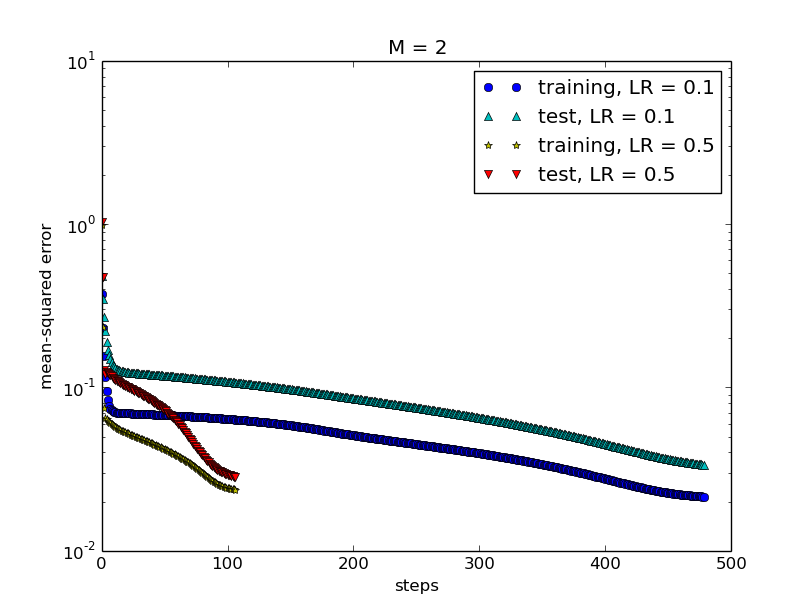
\includegraphics[width=.47\linewidth]{figures/course_of_learning1.png}
    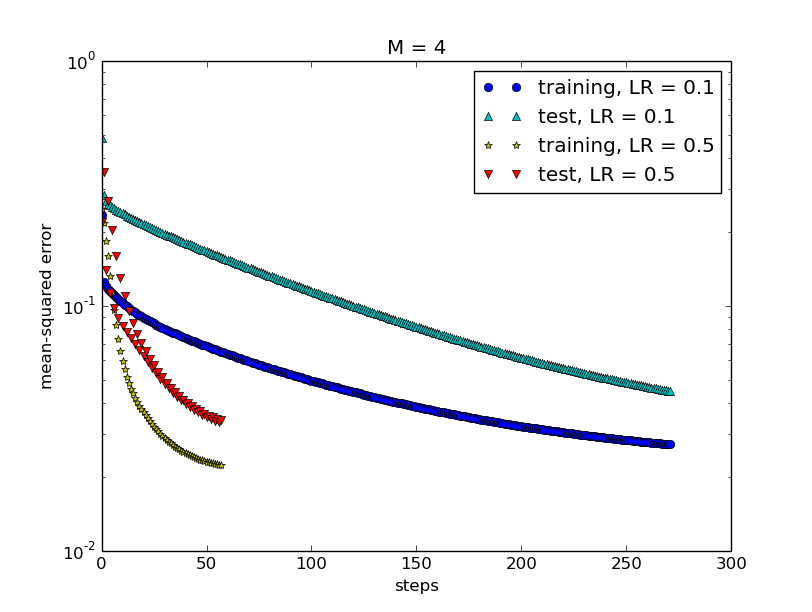
\includegraphics[width=.47\linewidth]{figures/course_of_learning2.png}
  \end{adjustwidth}
  \caption{Course of learning for different learning rates and number of hidden neurons.}
  \label{fig:course_of_learning}
\end{figure}

We picked the trained networked that obtained the best training error out of the four networks trained above. Figure \ref{fig:sinc} shows the real sinc-function plotted along with the output of this network.

\begin{figure}[H]
    \centering
    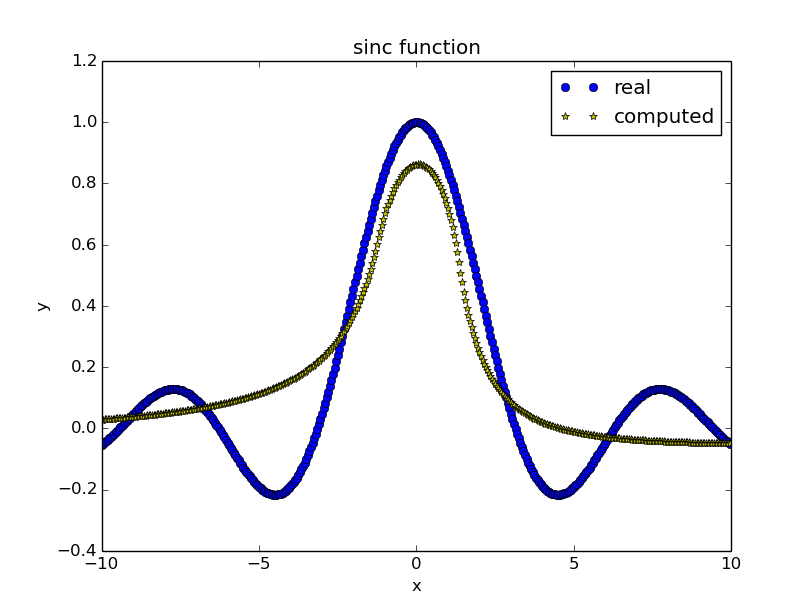
\includegraphics[width=.7\linewidth]{figures/sinc.png}
  \caption{The real sinc function and the sinc function computed using the network.}
  \label{fig:sinc}
\end{figure}

\section{Support Vector Machines}
\subsection{Data normalization}
After normalization of the training and test data sets, the following means and variances were computed for each feature of the sets
\begin{figure}[H]
	\begin{lstlisting}
	Training set, feature = 0: Mean = 8.50793358667e-16, variance = 1.0
	Training set, feature = 1: Mean = -6.29881634379e-16, variance = 1.0
	Training set, feature = 2: Mean = 3.85179416707e-17, variance = 1.0
	Training set, feature = 3: Mean = 3.21738101014e-16, variance = 1.0
	Training set, feature = 4: Mean = -1.05641119435e-15, variance = 1.0
	Training set, feature = 5: Mean = -1.20085347561e-16, variance = 1.0
	Training set, feature = 6: Mean = 4.74676987059e-16, variance = 1.0
	Training set, feature = 7: Mean = 2.29974769387e-16, variance = 1.0
	Training set, feature = 8: Mean = 1.48860515751e-15, variance = 1.0
	Training set, feature = 9: Mean = -7.8055475915e-16, variance = 1.0
	Training set, feature = 10: Mean = 1.23597277537e-15, variance = 1.0
	Training set, feature = 11: Mean = -1.93722588991e-16, variance = 1.0
	Training set, feature = 12: Mean = 8.93842822887e-16, variance = 1.0
	Training set, feature = 13: Mean = -1.45008721584e-16, variance = 1.0
	Training set, feature = 14: Mean = 1.40477199034e-16, variance = 1.0
	Training set, feature = 15: Mean = -1.44442281265e-15, variance = 1.0
	Training set, feature = 16: Mean = 1.19179043052e-15, variance = 1.0
	Training set, feature = 17: Mean = 3.16158663875e-15, variance = 1.0
	Training set, feature = 18: Mean = -2.44305709449e-15, variance = 1.0
	Training set, feature = 19: Mean = 7.43169698116e-16, variance = 1.0
	Training set, feature = 20: Mean = -1.43705908851e-15, variance = 1.0
	Training set, feature = 21: Mean = -1.04225018638e-16, variance = 1.0
	Test set, feature = 0: Mean = -0.0785793098786, variance = 0.732185076092
	Test set, feature = 1: Mean = -0.158041615121, variance = 0.714913359501
	Test set, feature = 2: Mean = 0.0556231122134, variance = 0.797590331684
	Test set, feature = 3: Mean = 0.113183870596, variance = 1.99040213886
	Test set, feature = 4: Mean = 0.071573768538, variance = 1.66604029201
	Test set, feature = 5: Mean = 0.0869148906279, variance = 2.13673680831
	Test set, feature = 6: Mean = 0.11567238855, variance = 1.92226228418
	Test set, feature = 7: Mean = 0.0870155300787, variance = 2.13767335461
	Test set, feature = 8: Mean = 0.248982135224, variance = 1.77195651078	
	Test set, feature = 9: Mean = 0.2451873402, variance = 1.82895633206
	Test set, feature = 10: Mean = 0.22956619607, variance = 1.71731489777
	Test set, feature = 11: Mean = 0.250890507791, variance = 1.77783879058
	Test set, feature = 12: Mean = 0.316608257189, variance = 2.1902285482
	Test set, feature = 13: Mean = 0.229602833976, variance = 1.71745429545
	Test set, feature = 14: Mean = 0.149057020979, variance = 2.66297001969
	Test set, feature = 15: Mean = -0.0567634602313, variance = 1.36090146496
	Test set, feature = 16: Mean = 0.0735676557785, variance = 1.08263292728
	Test set, feature = 17: Mean = 0.0867669827243, variance = 0.951308458665
	Test set, feature = 18: Mean = 0.154772446101, variance = 1.21651004673
	Test set, feature = 19: Mean = 0.310694549709, variance = 1.36280271312
	Test set, feature = 20: Mean = 0.087416429507, variance = 1.13351688737
	Test set, feature = 21: Mean = 0.168576603142, variance = 1.41470112481
	\end{lstlisting}
	\caption{Mean and variances of normalized data sets}
	\label{fig:mean_variance_data}
\end{figure}

\subsection{Model using grid-search}
\subsubsection{Implementation}
In order to utilize grid-search and determine appropriate SVM hyperparameters $\gamma$ and $C$, the python library \texttt{scikit-learn}\footnote{\url{http://scikit-learn.org/}} was used. The library features an SVM implementation, which is documented in the following link: \url{http://scikit-learn.org/stable/modules/svm.html}.\\

The SVM hyperparameters were calculating by iterating each combination of pairs of $\gamma$ and $C$ and performing 5-fold cross-validation on these pairs. The mean of the accuracies computed for each 5-fold cross-validation was stored along with its corresponding parameter pair. The appropriate SVM hyperparameter pair was then simply selected from the pair generating the smallest loss.

\subsubsection{Results}
The following hyperparameter configurations and accuracies were computed for the regular- and normalized dataset.

\begin{figure}[H]
	\begin{lstlisting}
	Training set: Hyperparameter config = (1, 0.001)
	Training set: Accuracy = 0.810526315789
	Test set: Accuracy = 0.824742268041
	Normalized Training set: Hyperparameter config = (1, 0.01)
	Normalized Training set: Accuracy = 0.884210526316
	Normalized Test set: Accuracy = 0.865979381443
	\end{lstlisting}
	\caption{Appropriate hyperparameter configurations and corresponding accuracies}
	\label{fig:grid_search_results}
\end{figure}

As seen in ~\ref{fig:grid_search_results}, the normalized data sets resulted in more accurate classifications and reported a different best hyperparameter configuration, compared to the non-normalized training set. The normalized data set performs better in SVM model selection due to how scaling affects SVM. The variances affects the margin of the SVM and thus by scaling these down through normalization, these impact the margin less, resulting in better accuracies and a different model selection from the grid search.

\subsection{Inspecting the kernel expansion}
\subsubsection{Support vectors}
For the purpose of calculating bounded and free support vectors, the \texttt{scikit-learn} library was utilized again. After fitting the test data set, the number of bounded and free support vectors were found for various values of $C$ by inspecting the \texttt{dual\_coef\_} variable generated by the SVM implementation, which resulted in the following number of bounded and free support vectors
\begin{figure}[H]
	\begin{lstlisting}
	C = 0.1 	 bounded support vectors: 25 	 free support vectors: 57
	C = 1.0 	 bounded support vectors: 23 	 free support vectors: 60
	C = 10.0 	 bounded support vectors: 0 	 free support vectors: 79
	C = 100.0 	 bounded support vectors: 0 	 free support vectors: 79
	C = 1000.0 	 bounded support vectors: 0 	 free support vectors: 79
	\end{lstlisting}
	\caption{Number of bounded and free support vectors for varying values of $C$}
	\label{fig:free_bounded}
\end{figure}

As shown in ~\ref{fig:free_bounded}, the value of $C$ affects the misclassification rate of the training examples. For small values of C a large-margin hyperplane will be used regardless of the misclassification rate. For larger values of C, the SVM will pick a smaller-margin hyperplane provided it minimizes the misclassification rate. 

\subsubsection{Scaling behaviour}
Training an SVM takes quadratic time with respect to the number of training examples or even cubic time in the worst case scenario. For very large training sets the time it takes to train the SVM will be impractical. The number of support vectors used will be determined by how large the Bayes risk is for the given problem. With a very large risk the number of support vectors might follow the number of training examples closely.

\end{document}
